% Shared TikZ diagrams and colours for the paradise reports (Phase 1 and Phase 2)
\usepackage{tikz}
\usetikzlibrary{arrows.meta,calc,fit,positioning,shapes.geometric}

\definecolor{lmNavy}{HTML}{1B3A4B}
\definecolor{lmTeal}{HTML}{2A9D8F}
\definecolor{lmSand}{HTML}{E9C46A}
\definecolor{lmCoral}{HTML}{E76F51}
\definecolor{lmInk}{HTML}{264653}
\definecolor{lmMist}{HTML}{F4F1DE}
\definecolor{lmBlue}{HTML}{3D5A80}
\definecolor{lmPurple}{HTML}{7B5EA7}
\definecolor{lmGreen}{HTML}{2F855A}
\definecolor{lmAmber}{HTML}{B7791F}
\definecolor{lmRed}{HTML}{C53030}

% ---------- Phase 1: request path, left to right ----------
\newcommand{\drawRequestPath}{%
\begin{tikzpicture}[font=\sffamily\tiny, node distance=0.35cm and 0.28cm]
  \tikzset{s/.style={draw=##1, fill=##1!14, rounded corners=2pt, align=center,
           inner sep=4pt, minimum height=1.15cm, minimum width=2.25cm, line width=0.7pt}}
  \node[s=lmNavy] (1) {1. DNS query\\UDP/53\\to Mac 1 (dnsmasq)};
  \node[s=lmTeal, right=of 1] (2) {2. A record\\app.paradise.test\\$\to$ edge IP (Mac 2)};
  \node[s=lmBlue, right=of 2] (3) {3. TCP\\SYN / SYN-ACK / ACK\\:443};
  \node[s=lmSand, right=of 3] (4) {4. TLS 1.3\\SNI + team CA\\terminates at Mac 2};
  \node[s=lmCoral, right=of 4] (5) {5. HTTP/2 $\to$ HTTP/1.1\\round robin to\\:3001 (A) / :3002 (B)};
  \foreach \a/\b in {1/2,2/3,3/4,4/5}
    \draw[-{Latex}, thick, lmInk] (\a) -- (\b);
\end{tikzpicture}%
}

% ---------- Phase 1: two independent TCP connections ----------
\newcommand{\drawTwoConnections}{%
\begin{tikzpicture}[font=\sffamily\scriptsize]
  \tikzset{m/.style={draw=##1, fill=##1!12, rounded corners=3pt, align=center,
           inner sep=5pt, minimum width=3.0cm, minimum height=1.25cm, line width=0.8pt}}
  \node[m=lmSand, text=lmInk] (c) at (0,0) {\textbf{Client}\\curl / browser\\ephemeral port};
  \node[m=lmTeal] (e) at (6,0) {\textbf{Mac 2 edge}\\nginx :443\\TLS ends here};
  \node[m=lmBlue] (a) at (12.6,1.5) {\textbf{Mac 3 Backend A}\\Express :3001};
  \node[m=lmCoral] (b) at (12.6,-1.5) {\textbf{Mac 4 Backend B}\\Express :3002};
  \draw[-{Latex}, very thick, lmTeal] (c) -- (e);
  \node[align=center, text=lmTeal, font=\sffamily\scriptsize] at (3,0.95) {connection 1: HTTPS\\\textbf{encrypted} (TLS 1.3, HTTP/2)};
  \draw[-{Latex}, thick, lmBlue] (e.east) -- (a.west);
  \draw[-{Latex}, thick, lmCoral] (e.east) -- (b.west);
  \node[align=center, text=lmInk, font=\sffamily\scriptsize] at (12.6,0) {connection 2: plain HTTP/1.1\\pooled (\texttt{keepalive 16})};
\end{tikzpicture}%
}

% ---------- Phase 1: TLS trust chain ----------
\newcommand{\drawTls}{%
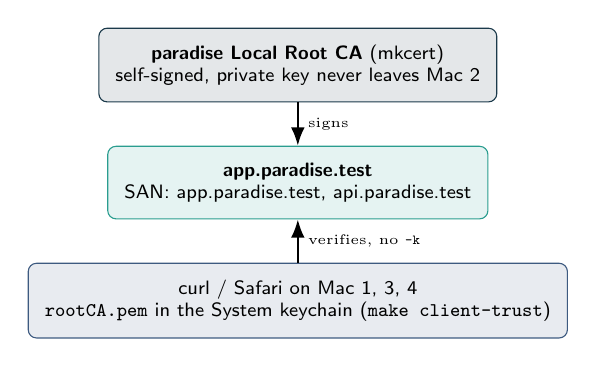
\begin{tikzpicture}[font=\sffamily\scriptsize, node distance=0.55cm]
  \node[draw=lmNavy, fill=lmNavy!12, rounded corners=3pt, align=center, inner sep=6pt] (ca)
    {\textbf{paradise Local Root CA} (mkcert)\\self-signed, private key never leaves Mac 2};
  \node[draw=lmTeal, fill=lmTeal!12, rounded corners=3pt, align=center, inner sep=6pt, below=of ca] (srv)
    {\textbf{app.paradise.test}\\SAN: app.paradise.test, api.paradise.test};
  \node[draw=lmBlue, fill=lmBlue!12, rounded corners=3pt, align=center, inner sep=6pt, below=of srv] (cli)
    {curl / Safari on Mac 1, 3, 4\\\texttt{rootCA.pem} in the System keychain (\texttt{make client-trust})};
  \draw[-{Latex}, thick] (ca) -- node[right, font=\tiny] {signs} (srv);
  \draw[-{Latex}, thick] (cli) -- node[right, font=\tiny] {verifies, no \texttt{-k}} (srv);
\end{tikzpicture}%
}

% ---------- Phase 1: OSI mapping ----------
\newcommand{\drawOsi}{%
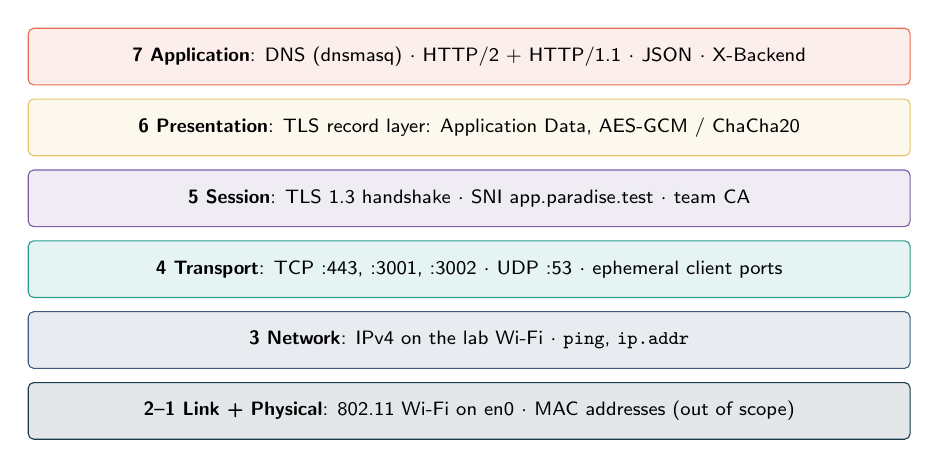
\begin{tikzpicture}[font=\sffamily\scriptsize]
  \foreach \y/\c/\t/\n in {
    5.1/lmCoral/7 Application/{DNS (dnsmasq) $\cdot$ HTTP/2 + HTTP/1.1 $\cdot$ JSON $\cdot$ X-Backend},
    4.2/lmSand/6 Presentation/{TLS record layer: Application Data, AES-GCM / ChaCha20},
    3.3/lmPurple/5 Session/{TLS 1.3 handshake $\cdot$ SNI app.paradise.test $\cdot$ team CA},
    2.4/lmTeal/4 Transport/{TCP :443, :3001, :3002 $\cdot$ UDP :53 $\cdot$ ephemeral client ports},
    1.5/lmBlue/3 Network/{IPv4 on the lab Wi-Fi $\cdot$ \texttt{ping}, \texttt{ip.addr}},
    0.6/lmNavy/2--1 Link + Physical/{802.11 Wi-Fi on en0 $\cdot$ MAC addresses (out of scope)}
  } {
    \node[draw=\c, fill=\c!12, rounded corners=2pt, minimum width=11.2cm,
          minimum height=0.72cm, anchor=west] at (0,\y) {\textbf{\t}: \n};
  }
\end{tikzpicture}%
}

% ---------- Phase 1 + 2: top-down diagnosis ladder ----------
\newcommand{\drawDiagnose}{%
\begin{tikzpicture}[font=\sffamily\scriptsize, node distance=0.22cm]
  \tikzset{st/.style={draw=##1, fill=##1!12, rounded corners=2pt, align=left,
           inner sep=4pt, text width=5.1cm, minimum height=0.62cm, anchor=west, line width=0.7pt},
           ff/.style={font=\sffamily\tiny, align=left, anchor=west, text=lmInk}}
  \node[st=lmNavy]   (l0) at (0,0)     {\textbf{0 Local config}\quad resolvers, /etc/hosts};
  \node[st=lmCoral]  (l1) at (0,-0.85) {\textbf{1 DNS}\quad \texttt{dig @primary}, \texttt{@backup}};
  \node[st=lmBlue]   (l2) at (0,-1.7)  {\textbf{2 Network}\quad \texttt{ping <ip>}};
  \node[st=lmTeal]   (l3) at (0,-2.55) {\textbf{3 Transport}\quad TCP connect :443};
  \node[st=lmPurple] (l4) at (0,-3.4)  {\textbf{4 TLS}\quad \texttt{curl -v} without \texttt{-k}};
  \node[st=lmSand]   (l5) at (0,-4.25) {\textbf{5 HTTP}\quad \texttt{curl -i}};
  \foreach \a/\b in {l0/l1,l1/l2,l2/l3,l3/l4,l4/l5}
    \draw[-{Latex}, thick, lmInk] (\a.south west) ++(0.35,0) -- ++(0,-0.23);
  \node[ff] at (5.7,0)     {wrong resolver $\Rightarrow$ the client never asks Mac 1};
  \node[ff] at (5.7,-0.85) {NXDOMAIN / timeout / an IP that is not an edge};
  \node[ff] at (5.7,-1.7)  {host unreachable (a sleeping Mac may still reply)};
  \node[ff] at (5.7,-2.55) {\textbf{refused} = no listener (RST) $\cdot$ \textbf{timeout} = dropped};
  \node[ff] at (5.7,-3.4)  {curl 60 = CA not trusted $\cdot$ curl 35 = handshake failure};
  \node[ff] at (5.7,-4.25) {502 / 504 = edge up, backends not};
  \draw[lmRed, thick, -{Latex}] (-0.45,0.2) -- node[left, rotate=90, anchor=south, font=\sffamily\tiny, text=lmRed] {stop at the first failure} (-0.45,-4.45);
\end{tikzpicture}%
}

% ---------- Phase 2: keep-alive timer race (Incident 2) ----------
\newcommand{\drawKeepalive}{%
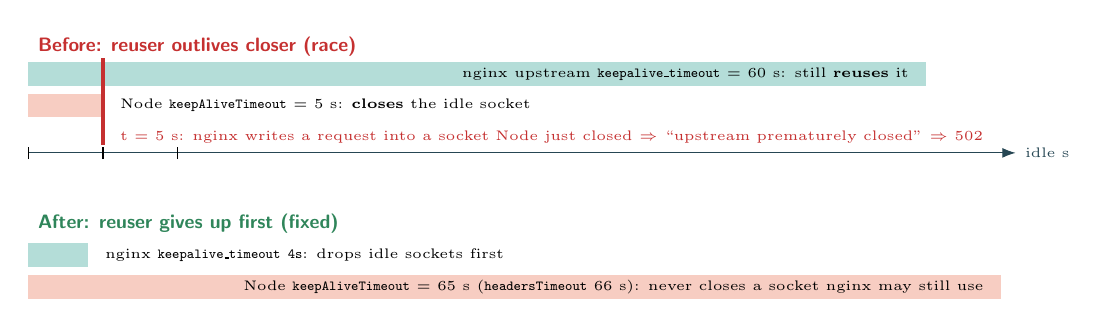
\begin{tikzpicture}[font=\sffamily\scriptsize, x=0.95cm]
  % before
  \node[anchor=west, font=\sffamily\bfseries\scriptsize, text=lmRed] at (0,2.55) {Before: reuser outlives closer (race)};
  \draw[lmInk, -{Latex}] (0,1.2) -- (13.2,1.2) node[right, font=\tiny] {idle s};
  \foreach \x in {0,5,10} \draw (\x*0.2,1.12) -- (\x*0.2,1.28);
  \fill[lmCoral!35] (0,1.65) rectangle (1.0,1.95);
  \node[anchor=west, font=\tiny] at (1.1,1.8) {Node \texttt{keepAliveTimeout} = 5 s: \textbf{closes} the idle socket};
  \fill[lmTeal!35] (0,2.05) rectangle (12,2.35);
  \node[anchor=east, font=\tiny] at (11.9,2.2) {nginx upstream \texttt{keepalive\_timeout} = 60 s: still \textbf{reuses} it};
  \draw[lmRed, very thick] (1.0,1.3) -- (1.0,2.4);
  \node[font=\tiny, text=lmRed, align=left, anchor=west] at (1.1,1.4) {t = 5 s: nginx writes a request into a socket Node just closed $\Rightarrow$ ``upstream prematurely closed'' $\Rightarrow$ 502};
  % after
  \node[anchor=west, font=\sffamily\bfseries\scriptsize, text=lmGreen] at (0,0.3) {After: reuser gives up first (fixed)};
  \fill[lmTeal!35] (0,-0.25) rectangle (0.8,0.05);
  \node[anchor=west, font=\tiny] at (0.9,-0.1) {nginx \texttt{keepalive\_timeout 4s}: drops idle sockets first};
  \fill[lmCoral!35] (0,-0.65) rectangle (13.0,-0.35);
  \node[anchor=east, font=\tiny] at (12.9,-0.5) {Node \texttt{keepAliveTimeout} = 65 s (\texttt{headersTimeout} 66 s): never closes a socket nginx may still use};
\end{tikzpicture}%
}

% ---------- Phase 2: CLOSED vs FILTERED ----------
\newcommand{\drawFiltered}{%
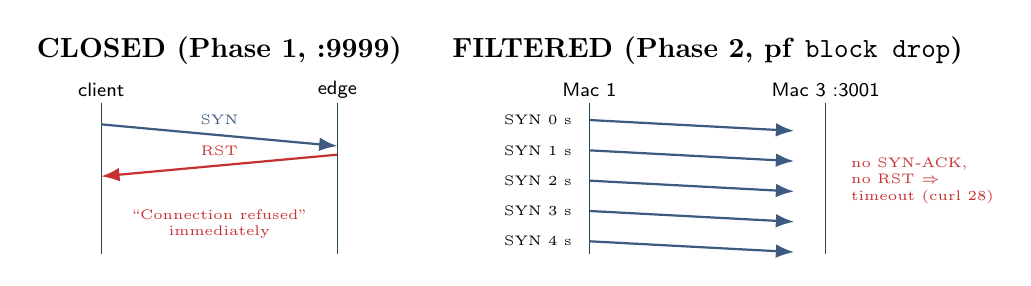
\begin{tikzpicture}[font=\sffamily\scriptsize, y=0.55cm]
  \node[font=\bfseries] at (1.5,6.2) {CLOSED (Phase 1, :9999)};
  \node at (0,5.3) {client}; \node at (3,5.3) {edge};
  \draw[lmInk] (0,5) -- (0,1.5); \draw[lmInk] (3,5) -- (3,1.5);
  \draw[-{Latex}, thick, lmBlue] (0,4.5) -- node[above, font=\tiny] {SYN} (3,4.0);
  \draw[-{Latex}, thick, lmRed] (3,3.8) -- node[above, font=\tiny] {RST} (0,3.3);
  \node[font=\tiny, align=center, text=lmRed] at (1.5,2.2) {``Connection refused''\\immediately};
  \begin{scope}[xshift=6.2cm]
  \node[font=\bfseries] at (1.5,6.2) {FILTERED (Phase 2, pf \texttt{block drop})};
  \node at (0,5.3) {Mac 1}; \node at (3,5.3) {Mac 3 :3001};
  \draw[lmInk] (0,5) -- (0,1.5); \draw[lmInk] (3,5) -- (3,1.5);
  \foreach \y/\t in {4.6/0 s,3.9/1 s,3.2/2 s,2.5/3 s,1.8/4 s}
    { \draw[-{Latex}, thick, lmBlue] (0,\y) -- (2.6,\y-0.25); \node[font=\tiny, anchor=east] at (-0.1,\y) {SYN \t}; }
  \node[font=\tiny, align=left, anchor=west, text=lmRed] at (3.2,3.2) {no SYN-ACK,\\no RST $\Rightarrow$\\timeout (curl 28)};
  \end{scope}
\end{tikzpicture}%
}
